\documentclass[11pt,a4paper,twoside]{article}%
\usepackage{graphicx}
\usepackage{tikz}
\usepackage{amsmath}
\usepackage{amsfonts}
\usepackage{amssymb}
\usepackage{epstopdf}
\usepackage[latin1]{inputenc}
\setcounter{MaxMatrixCols}{30}
%TCIDATA{OutputFilter=latex2.dll}
%TCIDATA{Version=5.50.0.2953}
%TCIDATA{CSTFile=40 LaTeX article.cst}
%TCIDATA{Created=Thursday, December 26, 2013 11:29:10}
%TCIDATA{LastRevised=Friday, March 28, 2014 14:13:05}
%TCIDATA{<META NAME="GraphicsSave" CONTENT="32">}
%TCIDATA{<META NAME="SaveForMode" CONTENT="1">}
%TCIDATA{BibliographyScheme=Manual}
%TCIDATA{<META NAME="DocumentShell" CONTENT="Standard LaTeX\Blank - Standard LaTeX Article">}
%BeginMSIPreambleData
\providecommand{\U}[1]{\protect\rule{.1in}{.1in}}
%EndMSIPreambleData
\newtheorem{theorem}{Theorem}
\newtheorem{acknowledgement}[theorem]{Acknowledgement}
\newtheorem{algorithm}[theorem]{Algorithm}
\newtheorem{axiom}[theorem]{Axiom}
\newtheorem{case}[theorem]{Case}
\newtheorem{claim}[theorem]{Claim}
\newtheorem{conclusion}[theorem]{Conclusion}
\newtheorem{condition}[theorem]{Condition}
\newtheorem{conjecture}[theorem]{Conjecture}
\newtheorem{corollary}[theorem]{Corollary}
\newtheorem{criterion}[theorem]{Criterion}
\newtheorem{definition}[theorem]{Definition}
\newtheorem{example}[theorem]{Example}
\newtheorem{exercise}[theorem]{Exercise}
\newtheorem{lemma}[theorem]{Lemma}
\newtheorem{notation}[theorem]{Notation}
\newtheorem{problem}[theorem]{Problem}
\newtheorem{proposition}[theorem]{Proposition}
\newtheorem{remark}[theorem]{Remark}
\newtheorem{solution}[theorem]{Solution}
\newtheorem{summary}[theorem]{Summary}
\newenvironment{proof}[1][Proof]{\noindent\textbf{#1.} }{\ \rule{0.5em}{0.5em}}
\topmargin -0.7in
\oddsidemargin -0.30in
\evensidemargin -0.7in
\textwidth 7.3in
\textheight 9.5in
\begin{document}

\begin{center}
\textbf{\textsf{Estad\'{\i}stica (Qu\'{\i}mica) - Primer Cuatrimestre 2020 - Coronavirus}}

\textbf{Pr\'{a}ctica 7 - An\'{a}lisis de la varianza}\vspace{-0.1in}

\end{center}

Comentario: En todos los ejercicios propuestos

\begin{enumerate}
\item[a)] defina las variables aleatorias y los par\'{a}metros involucrados.

\item[b)] de ser posible indique:

\begin{enumerate}
\item[i.] la distribuci\'{o}n de las variables aleatorias

\item[ii.] el significado intuitivo de los par\'{a}metros.

\item plantee las hip\'{o}tesis nula y alternativa, e indique el nivel que
usar\'{a} para el test. Elija un test, calcule el valor del estad\'{\i}stico,
calcule o acote el $p-$valor e indique la conclusi\'{o}n del test. Si el nivel
del test no se especifica en el enunciado, tome por default $0.05$. D\'{e} las
conclusiones en los t\'{e}rminos del problema.

\item compare los resultados de hacer las cuentas a mano con las salidas
obtenidas con el R, de manera de chequear las primeras y aprender a usar las
segundas, en aquellos ejercicios en los que ambas cosas sean posibles.
\end{enumerate}

\item Se analizaron 6 muestras de cada uno de tres tipos de cereal producidos
en cierta regi\'{o}n para determinar el contenido de tiamina. Los resultados
fueron los siguientes:%
\[
\text{%
\begin{tabular}
[c]{c|c|c|c|}\cline{2-4}
& Trigo & Ma\'{\i}z & Avena\\\cline{2-4}
& 5.2 & 6.5 & 9.3\\
& 4.5 & 8.0 & 7.1\\
& 6.0 & 6.1 & 8.8\\
& 6.1 & 7.5 & 8.0\\
& 6.7 & 5.9 & 6.5\\
& 5.8 & 5.6 & 8.2\\\hline
\multicolumn{1}{|c|}{media} & 5.72 & 6.60 & 7.98\\\hline
\multicolumn{1}{|c|}{desv\'{\i}o} & 0.77 & 0.95 & 1.04\\\hline
\end{tabular}
}%
\]


\begin{enumerate}
\item Suponga que se verifican los supuestos del modelo del An\'{a}lisis de la
Varianza. Construya la tabla y aplique el test $F$ para decidir si existen
diferencias en las medias del contenido de tiamina de los tres cereales a
nivel 0.05. Defina las variables aleatorias y los par\'{a}metros involucrados,
escriba el modelo bajo el cual vale el test $F$, establezca claramente las
hip\'{o}tesis de dicho test, d\'{e} el p-valor y escriba la conclusi\'{o}n.

\item Encuentre intervalos de confianza de nivel simult\'{a}neo 95\% para
todas las diferencias de medias. Utilice el m\'{e}todo que prefiera.
\textquestiondown Cu\'{a}ntas comparaciones de a pares pueden hacerse? Si en
el inciso (a) hall\'{o} diferencias significativas, detecte a partir de los
intervalos reci\'{e}n hallados cu\'{a}les son los cereales que difieren en sus
contenidos medios de tiamina, con nivel simult\'{a}neo 5\%.

\item Los precios de los cereales en el mercado son los siguientes%
\[%
\begin{tabular}
[c]{cc}%
Cereal & Precio (US\$/Tonelada)\\\hline
Avena & 313\\
Ma\'{\i}z & 223\\
Trigo & 198
\end{tabular}
\]
Se dispone de un presupuesto para comprar una gran cantidad de cereal. Se
desea comprar aquel cereal que tenga el mayor contenido medio poblacional de
tiamina, que se pueda pagar con dicho presupuesto. Bas\'andose en el resultado del
\'item anterior, decida qu\'e cereal comprar\'ia en cada una
de las siguientes situaciones:

\begin{enumerate}
\item Se puede gastar hasta US\$ 240 por tonelada, \textquestiondown cu\'{a}l
cereal prefiere?

\item Se puede gastar hasta US\$ 350 por tonelada, \textquestiondown cu\'{a}l
cereal prefiere?
\end{enumerate}
\end{enumerate}

\item En un experimento se midi\'{o} la p\'{e}rdida de humedad de 6 variedades
de sorgo sometidas a un cierto tratamiento. Sea $Y_{ij}$ la p\'{e}rdida de
humedad de la semilla $j$ de la variedad $i$. Considere el siguiente modelo:%
\[
Y_{ij}=\mu_{i}+\varepsilon_{ij}\qquad1\leq i\leq6,\text{ }1\leq j\leq8
\]
donde $\varepsilon_{ij}$\ son variables aleatorias independientes e
id\'{e}nticamente distribuidas y $\mu_{i}$ es la esperanza de la p\'{e}rdida
de humedad para la variedad $i$. Los datos obtenidos son los siguientes:%
\[
\text{%
\begin{tabular}
[c]{|c|c|c|c|c|c|}\hline
Var. 1 & Var. 2 & Var. 3 & Var. 4 & Var. 5 & Var. 6\\\hline
11.55 & 10.12 & 9.53 & 11.28 & 10.38 & 9.77\\
11.52 & 9.34 & 9.51 & 11.22 & 10.40 & 10.56\\
11.61 & 9.34 & 9.95 & 11.05 & 10.18 & 10.36\\
11.61 & 10.15 & 9.43 & 11.05 & 10.40 & 10.60\\
11.89 & 9.48 & 9.99 & 11.08 & 10.07 & 10.56\\
11.70 & 9.27 & 9.48 & 11.02 & 10.35 & 10.46\\
11.61 & 10.18 & 9.96 & 11.97 & 10.35 & 10.13\\
11.49 & 9.68 & 9.25 & 11.15 & 10.54 & 10.34\\\hline
\end{tabular}
}%
\]


\begin{enumerate}
\item Calcule las medias y los desv\'ios muestrales de cada variedad y analice mediante t\'ecnicas gr\'aficas si
existen diferencias entre las distintas variedades.


\item Suponga que se verifican los supuestos del modelo del An\'{a}lisis de la
Varianza. Construya la tabla y aplique el test $F$ para decidir si existen
diferencias entre las medias de p\'{e}rdida de humedad de las distintas
variedades a nivel 0.05.

\item Encuentre intervalos de confianza de nivel simult\'{a}neo 95\% para
todas las diferencias de medias. \textquestiondown Cu\'{a}ntas intervalos
(comparaciones de a pares) se pueden hacer?. Utilice el m\'{e}todo que
prefiera. Si en el inciso anterior hall\'{o} diferencias significativas,
detecte a partir de los intervalos reci\'{e}n hallados cu\'{a}les son las
variedades que difieren en sus p\'{e}rdidas medias de humedad, con nivel
simult\'{a}neo 5\%.

\item Calcule a mano el intervalo de confianza para la diferencia de medias
de las variedades 2 y 1.

\item Mirando los boxplots, \textquestiondown le parece v\'alido el supuesto de homogeneidad de varianzas? Aplicando el test
de Levene, \textquestiondown cu\'al es su conclusi\'on respecto a la homogeneidad de varianzas a nivel 20\%? \textquestiondown Encuentra
alguna contradicci\'on entre la conclusi\'on del boxplot y la del test? \textquestiondown Es v\'alido, entonces, usar el
modelo de anova para estudiar a estos datos?

\item Analice si es v\'alido el supuesto de normalidad haciendo un
histograma del conjunto de todos los residuos.
Aplicando el test de Shapiro Wilk, \textquestiondown  a qu\'e conclusi\'on llega?
Con esta nueva informaci\'on, utilice alguna herramienta que le permita confirmar 
(o dudar de) su conclusi\'on del inciso anterior respecto de la homoscedasticidad.

\end{enumerate}

\item Un experimento comenz\'{o} dividiendo un grupo de ratas de 20 d\'{\i}as
de edad en tres grupos al azar. Un grupo recibi\'{o} ATRO (atropina)
solamente, el segundo grupo recibi\'{o} SPI (spiroperidol) solamente y el
tercer grupo recibi\'{o} COMB (una combinaci\'{o}n de ambos). Una hora
despu\'{e}s que la droga fuera suministrada se midi\'{o} el tiempo en segundos
de reacci\'{o}n de cada rata ante un est\'{\i}mulo. Se obtuvieron los
siguientes tiempos de reacci\'{o}n en segundos:%
\[
\text{%
\begin{tabular}
[c]{c|c|c|c|}\cline{2-4}
& ATRO & COMB & SPI\\\cline{2-4}
& 10.5 & 16.0 & 35.8\\
& 0.8 & 5.9 & 10.5\\
& 0.7 & 11.5 & 10.5\\
& 0.7 & 4.4 & 5.2\\
& 0.3 & 17.7 & 20.9\\
& 5.8 & 13.5 & 44.2\\
&  & 2.3 & 20.7\\\hline
\multicolumn{1}{|c|}{media} & 2.000 & 16.413 & 20.925\\\hline
\multicolumn{1}{|c|}{desv\'{\i}o} & 3.7537 & 18.471 & 13.253\\\hline
\end{tabular}
}%
\]


\begin{enumerate}
\item Construya boxplots para los datos y describa las caracter\'{\i}sticas observadas.

\item \textquestiondown Es razonable suponer el modelo del An\'{a}lisis de la
Varianza a un factor para estos datos?

\item Intente aplicar el An\'{a}lisis de la Varianza y aplique el test de
Shapiro-Wilk a los residuos, \textquestiondown cu\'{a}l es la conclusi\'{o}n?

\item S\'{o}lo para comparar, calcule el valor p del test $F$ para estudiar la
hip\'{o}tesis de igualdad de medias (aunque no es correcto, \textquestiondown verdad?).

\item Aplique una transformaci\'{o}n logar\'{\i}tmica a los datos (calcule
$\log$ decimal para que todos lleguemos a los mismos resultados, pero
ser\'{\i}a equivalente calcular $\ln$ ya que difieren en una constante multiplicativa).

\item Repita (a), (b) y (c) pero con los datos transformados.

De ac\'{a} en adelante contin\'{u}e el an\'{a}lisis estad\'{\i}stico con los
datos originales o transformados, seg\'{u}n le parezca m\'{a}s conveniente.

\item Aplique el test $F$ para comparar las medias de los tres tratamientos.

\item En el caso de rechazar $H_{0}$ con el test $F$, detecte para cu\'{a}les
de las drogas las respuestas difieren significativamente.
\end{enumerate}

\item Se midieron las concentraciones de plasma (en nanogramos por mililitro)
de 10 perros sometidos a 3 tratamientos distintos. Las mediciones se presentan
en la siguiente tabla:%
\[
\text{%
\begin{tabular}
[c]{|c|cccccccccc|}\hline
Perro & 1 & 2 & 3 & 4 & 5 & 6 & 7 & 8 & 9 & 10\\\hline
Tratamiento 1 & 0.28 & 0.51 & 1.00 & 0.39 & 0.29 & 0.36 & 0.32 & 0.69 & 0.17 &
0.33\\
Tratamiento 2 & 0.30 & 0.39 & 0.63 & 0.68 & 0.38 & 0.21 & 0.88 & 0.39 & 0.51 &
0.32\\
Tratamiento 3 & 1.07 & 1.35 & 0.69 & 0.28 & 1.24 & 1.53 & 0.49 & 0.56 & 1.02 &
0.30\\\hline
\end{tabular}
}%
\]
Uno de los supuestos del modelo de ANOVA no es v\'alido en este caso. Sin hacer cuentas, responda cu\'al
y por qu\'e.

\item En un ensayo de colaboraci\'{o}n se envi\'{o} una muestra de una
sustancia que contiene olaquindox a tres laboratorios. Cada laboratorio
realiz\'{o} mediciones repetidas e independientes utilizando un detector
ultravioleta. Los resultados obtenidos se presentan en la siguiente tabla:%
\[
\text{%
\begin{tabular}
[c]{c|c|c|c|}\cline{2-4}
& Lab 1 & Lab 2 & Lab 3\\\cline{2-4}
& 21.0 & 26.5 & 21.2\\
& 23.8 & 27.1 & 21.4\\
& 23.0 & 25.9 & 22.6\\
& 22.1 & 26.2 & 23.7\\
& 22.8 & 25.6 & 21.9\\\hline
\multicolumn{1}{|c|}{media} & 22.54 & 26.26 & 22.16\\\hline
\multicolumn{1}{|c|}{desv\'{\i}o} & 1.05 & 0.58 & 1.02\\\hline
\end{tabular}
}%
\]


\begin{enumerate}
\item Mediante t\'{e}cnicas gr\'{a}ficas compare las mediciones obtenidas por
los tres laboratorios y describa lo que ve.

\item Plantee un modelo para analizar las diferencias entre laboratorios.
\textquestiondown Qu\'{e} supuestos debe hacer? \textquestiondown Puede
analizar la validez de los mismos? En caso de que su respuesta sea afirmativa, anal\'{\i}celos.

\item Escriba la tabla del An\'{a}lisis de la Varianza y aplique un test de la
hip\'{o}tesis de que los tres laboratorios miden con igual media, a un nivel
del 5\%.

\item \textquestiondown Se puede decir que la detecci\'on media de olaquindox de alg\'un laboratorio
es mayor o menor que la de los otros dos? Explique qu\'e m\'etodo utiliz\'o para llegar a la conclusi\'on.

\item Calcule los intervalos de confianza para las diferencias de medias entre
todos los pares de laboratorios.
\end{enumerate}

\item Sea $Y_{ij}=\mu_{i}+\varepsilon_{ij}$ con $1\leq i\leq I=3,$ $1\leq
j\leq J$, $\varepsilon_{ij}\sim N(0,\sigma^{2})$ independientes. Considere los
eventos
\begin{align*}
A_{1}  &  =\left\{  \mu_{1}-\mu_{2}\in\left[  a_{1},b_{1}\right]  \right\} \\
A_{2}  &  =\left\{  \mu_{1}-\mu_{3}\in\left[  a_{2},b_{2}\right]  \right\} \\
A_{3}  &  =\left\{  \mu_{2}-\mu_{3}\in\left[  a_{3},b_{3}\right]  \right\}
\end{align*}


\begin{enumerate}
\item Interprete los eventos $A_{1}$, $A_{2}$ y $A_{3}$ en el contexto de
intervalos de nivel simult\'{a}neo. Y tambi\'{e}n interprete el evento
$A_{1}\cap A_{2}\cap A_{3}.$

\item Hallar la probabilidad de $A_{1}\cap A_{2}\cap A_{3}$\ en el caso en el
que $A_{1}$, $A_{2}$ y $A_{3}$ sean eventos independientes.

\item Usando que
\[
P\left(  A_{1}^{c}\cup A_{2}^{c}\cup A_{3}^{c}\right)  \leq P\left(  A_{1}%
^{c}\right)  +P\left(  A_{2}^{c}\right)  +P\left(  A_{3}^{c}\right)  ,
\]
encontrar una cota inferior para $P\left(  A_{1}\cap A_{2}\cap A_{3}\right)  $
sin asumir independencia de los eventos $A_{i}$.

\item \textquestiondown C\'{o}mo se generalizar\'{\i}a si $I$ (la cantidad de
tratamientos o grupos a comparar) fuera mayor a 3? Pruebe que
\[
P\left(  \bigcap_{i=1}^{I}A_{i}\right)  \geq1-\sum_{i=1}^{I}P\left(  A_{i}%
^{c}\right)
\]
e interpr\'{e}telo.
\end{enumerate}

\item Se ha realizado un experimento para determinar si la densidad de un tipo
de ladrillo se ve afectada por la temperatura a la que es horneado. Para ello,
se cocieron 19 ladrillos a distintas temperaturas, obteni\'{e}ndose los
siguientes resultados:%
\[
\text{%
\begin{tabular}
[c]{l|ccccc}\hline
Temperatura & \multicolumn{5}{|c}{Densidad}\\\hline
Muy baja & 21.274 & 20.822 & 20.452 & 21.291 & 19.897\\
Baja & 22.309 & 23.999 & 23.304 & 21.532 & 22.783\\
Media & 24.010 & 23.132 & 23.848 & 22.300 & 23.153\\
Alta & 25.445 & 24.660 & 24.229 & 22.895 &
\end{tabular}
}%
\]
Por el modo en que fue llevado a cabo el experimento, se puede suponer
independencia entre las observaciones.

\begin{enumerate}
\item Se quiere aplicar el modelo de an\'{a}lisis de la varianza (ANOVA) para
decidir si existen diferencias en la densidad media de los distintos grupos.
El modelo de ANOVA\ para estos datos es

\vskip0.1in \makebox[\linewidth]{\dotfill}

donde las variables aleatorias y los par\'{a}metros involucrados son (def\'inalos con palabras)

\vskip0.1in \makebox[\linewidth]{\dotfill}\vskip0.1in
\makebox[\linewidth]{\dotfill}\vskip0.1in \makebox[\linewidth]{\dotfill}

Aqu\'{\i} $1\leq i\leq k=$ ..... y los $n_{i}$ son \ ......................................................................

Las hip\'{o}tesis que testea el ANOVA son

\makebox[\linewidth]{\dotfill}\vskip0.1in \makebox[\linewidth]{\dotfill}

\item Los supuestos necesarios para aplicar dicho modelo son \vskip0.1in
\makebox[\linewidth]{\dotfill} \vskip0.1in \makebox[\linewidth]{\dotfill}
\vskip0.1in \makebox[\linewidth]{\dotfill}

\item En base a los gr\'{a}ficos y salidas del R que se dan a
continuaci\'{o}n, decidir si se cumplen los supuestos del modelo de
an\'{a}lisis de la varianza. Indique qu\'{e} gr\'{a}fico o salida utiliza para
cada conclusi\'{o}n.\vskip0.1in \makebox[\linewidth]{\dotfill} \vskip0.1in
\makebox[\linewidth]{\dotfill} \vskip0.1in \makebox[\linewidth]{\dotfill}

\item En base a las salidas del R que se dan a continuaci\'on, completar la siguiente tabla de ANOVA, en los espacios recuadrados. Dar
las estimaciones de \textbf{todos} los par\'{a}metros del modelo que surjan
del ajuste de ANOVA.

\texttt{%
%TCIMACRO{\TEXTsymbol{>} }%
%BeginExpansion
$>$
%EndExpansion
salida%
%TCIMACRO{\TEXTsymbol{<}}%
%BeginExpansion
$<$%
%EndExpansion
-aov(densidad\symbol{126}temp.f)}

\texttt{%
%TCIMACRO{\TEXTsymbol{>} }%
%BeginExpansion
$>$
%EndExpansion
summary(salida)}

\texttt{\ \ \ \ \ \ \ \ \ \ \ \ \ Df \ \ \ \ \ \ Sum Sq \ \ \ \ Mean Sq
\ \ \ F value \ Pr(%
%TCIMACRO{\TEXTsymbol{>}}%
%BeginExpansion
$>$%
%EndExpansion
F) }

\texttt{temp.f \ \ \ \ \ \ \
\begin{tabular}
[c]{|c|}\hline
\ \ \\\hline
\end{tabular}
\ \ \ 31.169 \ \ \ \
\begin{tabular}
[c]{|c|}\hline
\texttt{ \ \ \ \ }\\\hline
\end{tabular}
\ \ \ 15.276 \ \ 7.894e-05 ***}

\texttt{Residuals \ \ \ \ 15 \ \ \ \
\begin{tabular}
[c]{|c|}\hline
\texttt{ \ \ \ \ }\\\hline
\end{tabular}
\ \ \ \ \ 0.6801 }

\vskip0.1in \makebox[\linewidth]{\dotfill} \vskip0.1in
\makebox[\linewidth]{\dotfill} \vskip0.1in \makebox[\linewidth]{\dotfill}

\item El estad\'{\i}stico utilizado para este test es (completar con una
f\'{o}rmula, explicando cada uno de los t\'{e}rminos involucrados en ella que
no haya definido anteriormente) \vskip0.1in \makebox[\linewidth]{\dotfill}
\vskip0.1in \makebox[\linewidth]{\dotfill} Su valor observado es \texttt{%
\begin{tabular}
[c]{|c|}\hline
\texttt{ \ \ \ \ \ \ \ \ \ \ }\\\hline
\end{tabular}
} y su pvalor resulta ser \texttt{%
\begin{tabular}
[c]{|c|}\hline
\ \ \ \ \ \ \ \ \ \ \ \\\hline
\end{tabular}
}.

Dar la conclusi\'{o}n del test cuyas hip\'{o}tesis exhibi\'{o} en (a), a nivel
0.05.\vskip0.1in \makebox[\linewidth]{\dotfill} \vskip0.1in \makebox[\linewidth]{\dotfill}

\item Se desean hacer comparaciones m\'{u}ltiples con el m\'{e}todo de
Bonferroni, para identificar cu\'{a}les son los grupos cuyas densidades medias
difieren, a nivel global 0.95. Indique cu\'{a}ntas comparaciones debe realizar
\texttt{%
\begin{tabular}
[c]{|c|}\hline
\ \ \ \ \ \ \ \ \ \ \ \\\hline
\end{tabular}
}. Los grados de libertad de la distribuci\'{o}n t involucrada en el
c\'{a}lculo del punto cr\'{\i}tico son \texttt{%
\begin{tabular}
[c]{|c|}\hline
\ \ \ \ \ \ \ \ \ \ \ \\\hline
\end{tabular}
}. Dicho punto cr\'{\i}tico corresponde al percentil \texttt{%
\begin{tabular}
[c]{|c|}\hline
\ \ \ \ \ \ \ \ \ \ \ \\\hline
\end{tabular}
} de la t. El valor cr\'{\i}tico de la t resulta ser 3.036. La f\'{o}rmula de
dichos intervalos de confianza es \vskip0.1in \makebox[\linewidth]{\dotfill}
Calcule los intervalos correspondientes a las comparaciones entre los grupos \vskip0.1in

\textquotedblleft alta\textquotedblright\ y \textquotedblleft muy
baja\textquotedblright\makebox[\linewidth]{\dotfill}\vskip0.1in
\textquotedblleft alta\textquotedblright\ y \textquotedblleft
baja\textquotedblright\makebox[\linewidth]{\dotfill}.

\item De las dos comparaciones entre grupos realizadas m\'as arriba,
\textquestiondown alguna de ellas permite concluir que las medias
poblacionales de los grupos correspondientes difieren entre s\'i a nivel conjunto 0.95?
\textquestiondown Cu\'al/es? Justifique
% 
% \item De las dos comparaciones entre grupos realizadas m\'{a}s arriba,
% \textquestiondown alguna de ellas permite concluir que las medias
% poblacionales de cu\'{a}les grupos difieren entre s\'{\i}, a nivel conjunto
% 0.95? Justifique.
\vskip0.1in \makebox[\linewidth]{\dotfill}\vskip0.1in \makebox[\linewidth]{\dotfill}
\end{enumerate}
\end{enumerate}

\texttt{%
%TCIMACRO{\TEXTsymbol{>} }%
%BeginExpansion
$>$
%EndExpansion
shapiro.test(residuals(salida))}

\texttt{\ Shapiro-Wilk normality test}

\texttt{data: residuals(salida) }

\texttt{W = 0.9621, p-value = 0.6143}

\texttt{%
%TCIMACRO{\TEXTsymbol{>} }%
%BeginExpansion
$>$
%EndExpansion
bartlett.test(densidad,temp.f)}

\texttt{ Bartlett test of homogeneity of variances}

\texttt{data: densidad and temp.f }

\texttt{Bartlett's K-squared = 1.4572, df = 3, p-value = 0.6922}

\texttt{%
%TCIMACRO{\TEXTsymbol{>} }%
%BeginExpansion
$>$
%EndExpansion
levene.test(densidad,temp.f)}

\texttt{ modified robust Brown-Forsythe Levene-type test based on the
absolute}

\texttt{ deviations from the median}

\texttt{data: densidad }

\texttt{Test Statistic = 0.4292, p-value = 0.735}

\texttt{%
%TCIMACRO{\TEXTsymbol{>} }%
%BeginExpansion
$>$
%EndExpansion
tapply(densidad, temp.f,mean)}

\texttt{ alta \ \ \ \ baja \ \ \ \ \ media \ \ \ \ muy baja }

\texttt{24.30725 \ 22.78540 \ 23.28860 \ \ 20.74720 }

\texttt{%
%TCIMACRO{\TEXTsymbol{>} }%
%BeginExpansion
$>$
%EndExpansion
tapply(densidad, temp.f,var)}

\texttt{ alta \ \ \ \ \ baja \ \ \ \ \ \ \ \ media \ \ \ \ muy baja }

\texttt{1.1398269 0.8849363 \ 0.4633968 0.3472037 }\newline

Los dos
gr\'{a}ficos que siguen son los boxplots de la densidad a distintas
temperaturas, y el qq-plot de los residuos del ajuste ANOVA.
%\[%
%%TCIMACRO{\FRAME{itbpF}{3.8969in}{3.8899in}{0in}{}{}{anovaboxplots.pdf}%
%%{\special{ language "Scientific Word";  type "GRAPHIC";
%%maintain-aspect-ratio TRUE;  display "USEDEF";  valid_file "F";
%%width 3.8969in;  height 3.8899in;  depth 0in;  original-width 6.979in;
%%original-height 6.9687in;  cropleft "0";  croptop "1";  cropright "1";
%%cropbottom "0";
%%filename '../parciales/segundoparcial/anovaboxplots.JPG';file-properties "XNPEU";}%
%%}}%
%%BeginExpansion
%{\includegraphics[
%natheight=6.968700in,
%natwidth=6.979000in,
%height=3.8899in,
%width=3.8969in
%]%
%{../parciales/segundoparcial/anovaboxplots.jpg}%
%}%
%%EndExpansion
%\]%
%\[%
%%TCIMACRO{\FRAME{itbpF}{3.8969in}{3.8899in}{0in}{}{}{anovaqqplots.eps}%
%%{\special{ language "Scientific Word";  type "GRAPHIC";
%%maintain-aspect-ratio TRUE;  display "USEDEF";  valid_file "F";
%%width 3.8969in;  height 3.8899in;  depth 0in;  original-width 6.979in;
%%original-height 6.9687in;  cropleft "0";  croptop "1";  cropright "1";
%%cropbottom "0";
%%filename '../parciales/segundoparcial/anovaqqplots.JPG';file-properties "XNPEU";}%
%%}}%
%%BeginExpansion
%{\includegraphics[
%natheight=6.968700in,
%natwidth=6.979000in,
%height=3.8899in,
%width=3.8969in
%]%
%{../parciales/segundoparcial/anovaqqplots.jpg}%
%}%
%%EndExpansion
%\]

{
\begin{tabular}[c]{cc}%
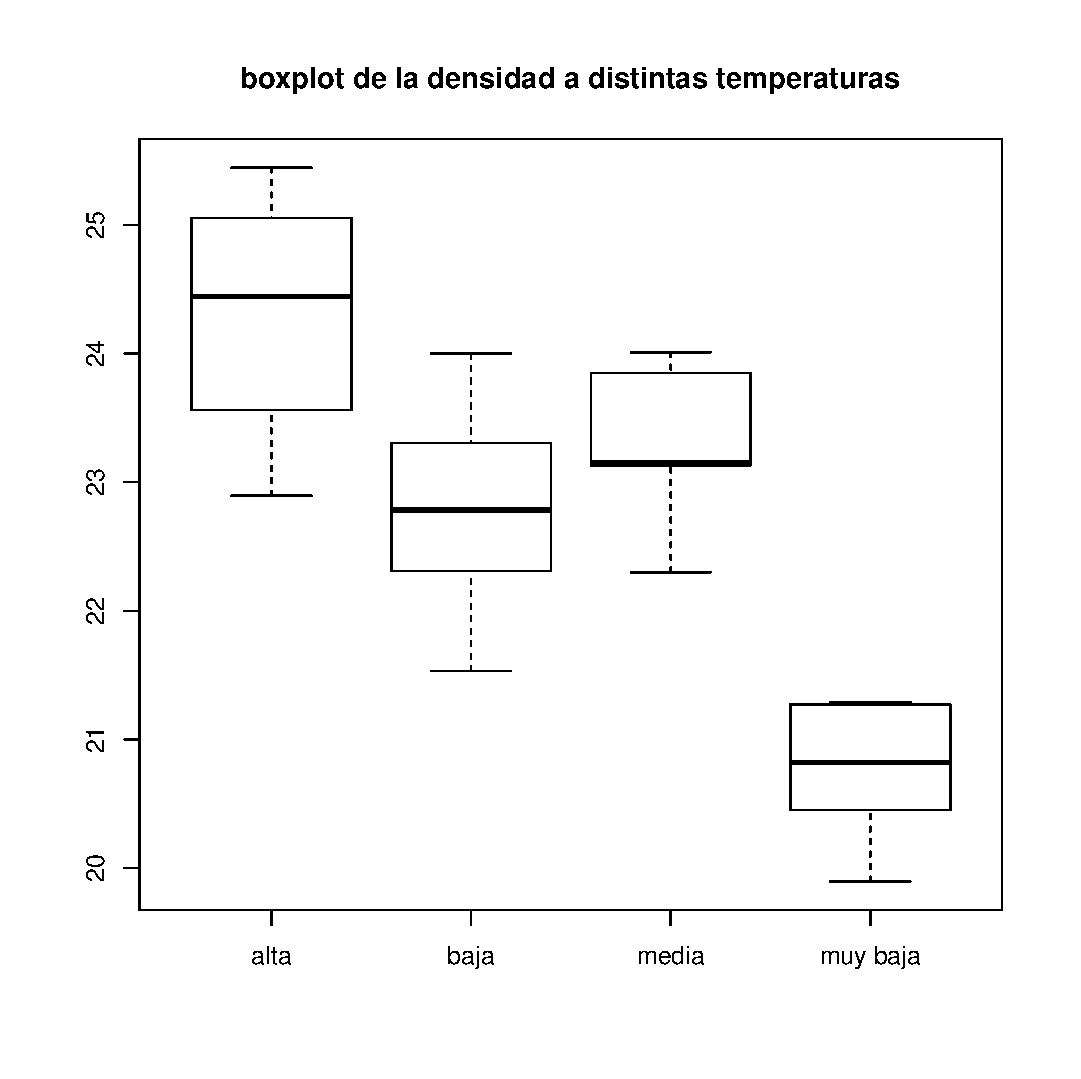
\includegraphics[scale=0.5]{anovaboxplots.eps} &
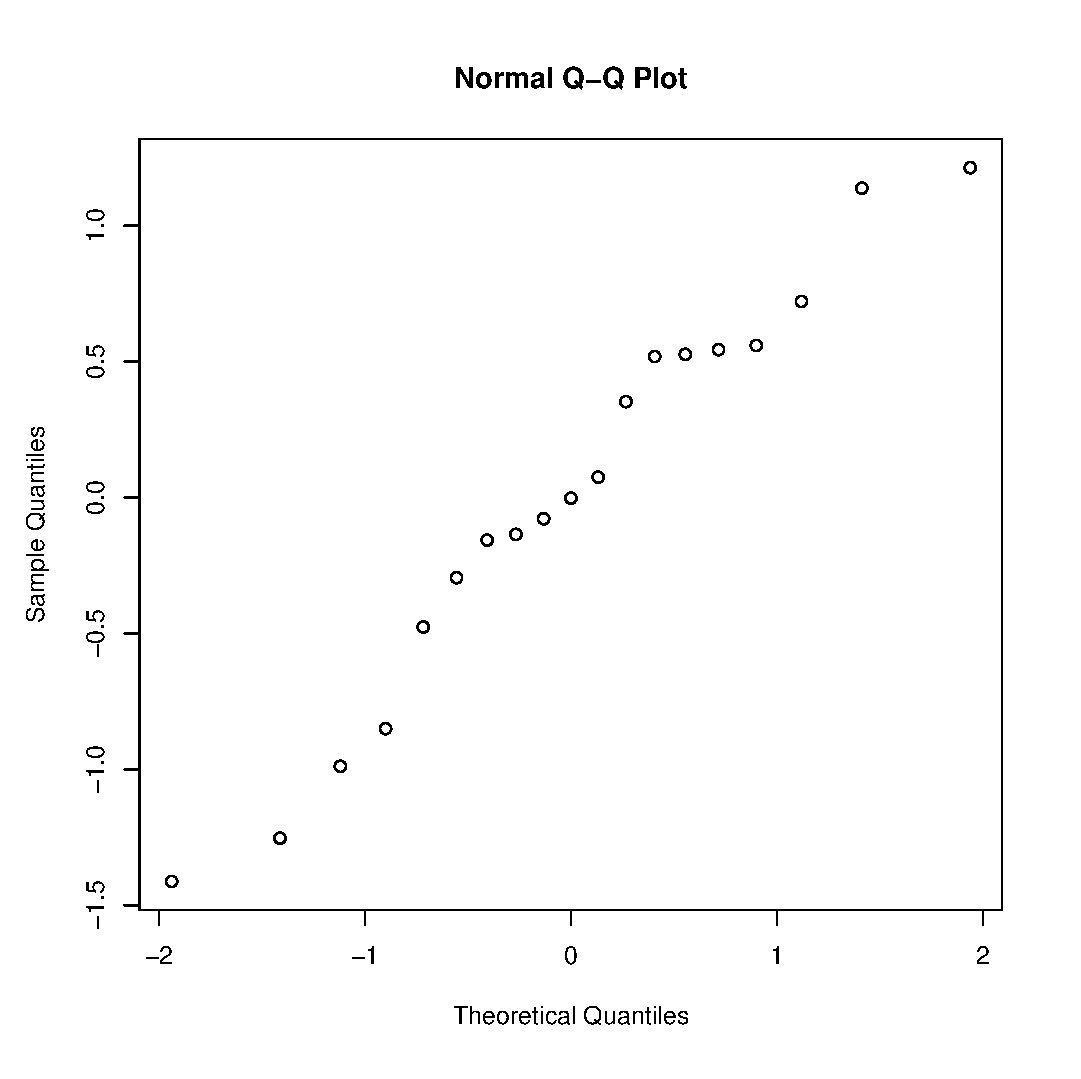
\includegraphics[scale=0.5]{anovaqqplots.eps}
\end{tabular}
}

\end{document}
